\documentclass{article}
\usepackage[utf8]{inputenc}
\usepackage{minted, graphicx, hyperref}

\begin{document}

\begin{center}
{\LARGE\bf COMP3013 Coursework: Design Report}\\
\vspace{2mm}
{\bf Matthew Lapointe, Takeaki Yamasaki, Zhengyi Yang}\\
\vspace{1mm}
\textbf{18th March 2016}
\end{center}

\section{YouTube Video}

\url{https://www.youtube.com/}

\section{Entity Relationship Diagram}

\begin{figure}[!h]
\begin{center}
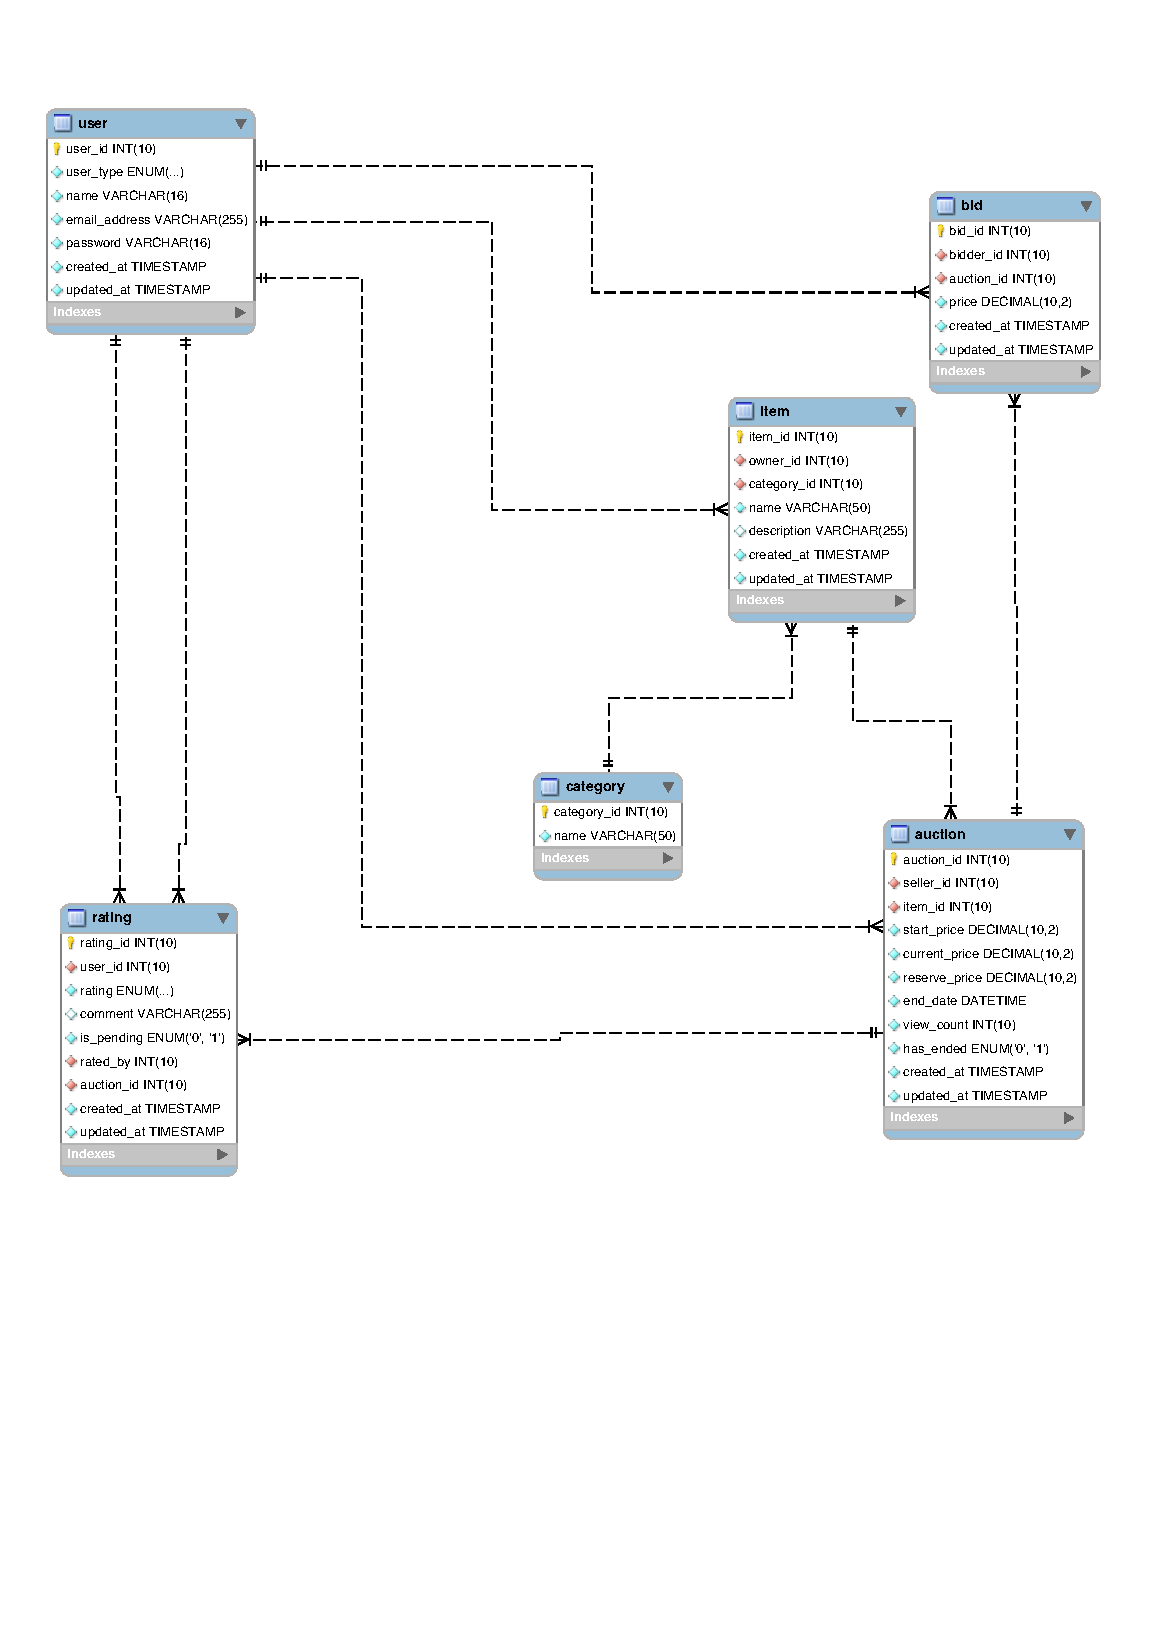
\includegraphics[scale=.65]{ERDiagram.pdf}
\end{center}
\end{figure}

\section{Database Schema}

user (\underline{user\_id}, user\_type, name, email\_address, password, created\_at, updated\_at)\\
\\
item (\underline{item\_id}, owner\_id \textbf{references} user(user\_id), category\_id \textbf{references} category(category\_id), name, description, created\_at, updated\_at)\\
\\
auction (\underline{auction\_id}, seller\_id \textbf{references} user(user\_id), item\_id \textbf{references} item(item\_id), start\_price, current\_price, reserve\_price, end\_date, view\_count, has\_ended, created\_at, updated\_at)\\
\\
bid (\underline{bid\_id}, bidder\_id \textbf{references} user(user\_id), auction\_id \textbf{references} auction(auction\_id), price, created\_at, updated\_at)\\
\\
category (\underline{category\_id}, name)\\
\\
rating (\underline{rating\_id}, user\_id \textbf{references} user(user\_id), rating, comment, is\_pending, rated\_by \textbf{references} user(user\_id), auction\_id \textbf{references} auction(auction\_id), created\_at, updated\_at)

\section{Normalisation Analysis}

\section{Database Queries}



\iffalse
\begin{minted}[]{java}
/**
 * Returns true if there are more elements to return from the array.
 *
 * @return true if there is a next element to return
 */
public boolean hasNext() {
    return index < endIndex;
}
\end{minted}
One of the mutants inserted into \texttt{ArrayIterator.java} is a negation of the return value for the function \texttt{hasNext()}.\\
\\
\texttt{ListUtils.java} contains the function shown above. One of the survived mutations negates the return value of the function, which indicated that perhaps there was not a test for this function.
\fi

\end{document}
